../cictikz/src/cictikz/data/tex/cictikz_preamble.tex

% What is left of each sensor's transfer after the best straight
% line, and what is left after also allowing a T ln T term - the bandgap
% curvature the references chapter warns about. Almost all of GR06's
% residual is that curvature; almost none of GR07's is.
%
% Generated by py/tikzplot.py. Edit the script in ex/ that
% produced it and re-run that, not this file.

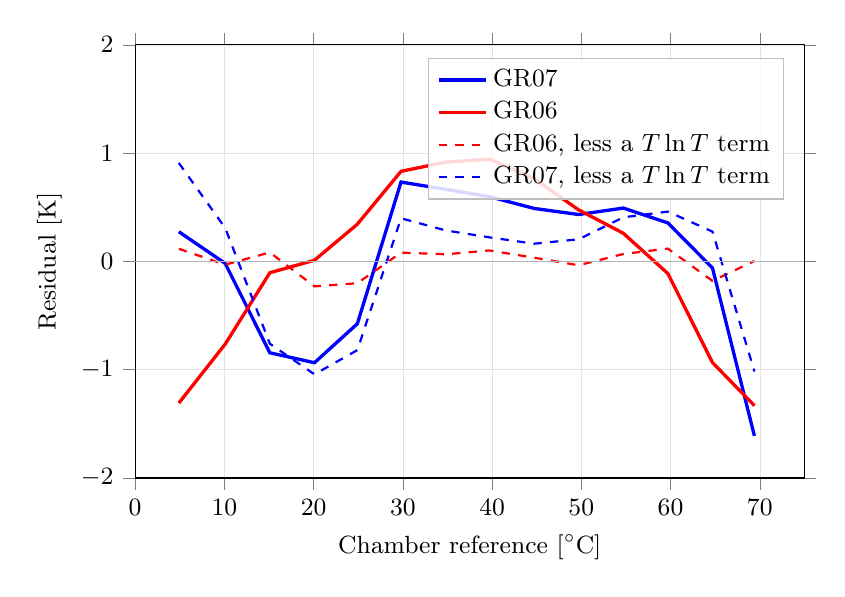
\begin{tikzpicture}[thick]

\begin{axis}[
  width=8.5cm,
  height=5.5cm,
  scale only axis,
  grid=both,
  grid style={gray!22, very thin},
  tick align=outside,
  tick label style={font=\small},
  label style={font=\small},
  title style={font=\small, yshift=-1mm},
  legend cell align=left,
  legend style={font=\small, draw=gray!50, fill=white, fill opacity=0.85, text opacity=1},
  xlabel={Chamber reference [$^\circ$C]},
  ylabel={Residual [K]},
  xmin=0,
  xmax=75,
  ymin=-2,
  ymax=2,
  legend pos=north east
]
\addplot[blue, very thick, mark=none] coordinates {(4.9,0.2746) (10.1,-0.0183) (15.1,-0.8436) (20.1,-0.9354) (24.9,-0.5759) (29.8,0.7333) (34.8,0.6659) (39.7,0.5987) (44.7,0.4898) (49.7,0.4335) (54.7,0.4931) (59.7,0.3561) (64.7,-0.0607) (69.4,-1.6113)};
\addlegendentry{GR07}
\addplot[red, very thick, mark=none] coordinates {(4.9,-1.3081) (10.1,-0.7629) (15.1,-0.1042) (20.1,0.0113) (24.9,0.3437) (29.8,0.8325) (34.8,0.917) (39.7,0.9453) (44.7,0.7651) (49.7,0.4766) (54.7,0.2609) (59.7,-0.1115) (64.7,-0.934) (69.4,-1.3316)};
\addlegendentry{GR06}
\addplot[red, thick, dashed, mark=none] coordinates {(4.9,0.11677) (10.1,-0.029734) (15.1,0.083238) (20.1,-0.23036) (24.9,-0.20107) (29.8,0.081735) (34.8,0.065997) (39.7,0.10153) (44.7,0.034699) (49.7,-0.035229) (54.7,0.068801) (59.7,0.11874) (64.7,-0.1799) (69.4,0.004788)};
\addlegendentry{GR06, less a $T\ln T$ term}
\addplot[blue, thick, dashed, mark=none] coordinates {(4.9,0.90963) (10.1,0.30848) (15.1,-0.75974) (20.1,-1.0426) (24.9,-0.81927) (29.8,0.39863) (34.8,0.28663) (39.7,0.22267) (44.7,0.16389) (49.7,0.20459) (54.7,0.40749) (59.7,0.46037) (64.7,0.2756) (69.4,-1.0164)};
\addlegendentry{GR07, less a $T\ln T$ term}
\draw[gray!60, thin] ({rel axis cs:0,0} |- {axis cs:0,0}) -- ({rel axis cs:1,0} |- {axis cs:0,0});
\end{axis}

\end{tikzpicture}
\end{document}
